% $Header: /Users/joseph/Documents/LaTeX/beamer/solutions/conference-talks/conference-ornate-20min.en.tex,v 90e850259b8b 2007/01/28 20:48:30 tantau $

\documentclass{beamer}

\usefonttheme{professionalfonts}%  don't change fonts inside beamer
% This file is a solution template for:

% - Talk at a conference/colloquium.
% - Talk length is about 20min.
% - Style is ornate.



% Copyright 2004 by Till Tantau <tantau@users.sourceforge.net>.
%
% In principle, this file can be redistributed and/or modified under
% the terms of the GNU Public License, version 2.
%
% However, this file is supposed to be a template to be modified
% for your own needs. For this reason, if you use this file as a
% template and not specifically distribute it as part of a another
% package/program, I grant the extra permission to freely copy and
% modify this file as you see fit and even to delete this copyright
% notice. 


\mode<presentation>
{
  % \usetheme{Warsaw}
  % or ...

  \setbeamercovered{transparent}
  % or whatever (possibly just delete it)
}


%\usepackage[english]{babel}
% or whatever

%\usepackage[latin1]{inputenc}
% or whatever
\usepackage{polyglossia}
\setmainlanguage{english}
\usepackage{fontspec}
\usepackage{xeCJK}
\usepackage{unicode-math}
	\setmathfont{Latin Modern Math} % default
	%\setmathfont[range=\mathalpha]{Asana Math}
	\setmathfont{Asana Math}[range={\mathbin}] %\mathord
	\setmathfont{STIX Math}[range={"02609}] % ☉
	\setmathfont{XITS Math}[range={"1D4B6-"1D4CF}] % Script, Latin, lowercase
	\setmathfont{Latin Modern Math}[range={"1D608-"1D63B}, sans-style=italic]
	\setmathfont{Latin Modern Math}[range={
		"00391-"003A9,
		"003B1-"003F5, 
		"1D6A8-"1D6E1},	% Bold Greek
		sans-style=upright]
		
	%\setmathfont{⟨font name⟩}[range=⟨unicode range⟩,⟨font features⟩]
\usepackage{siunitx}
% ':=' as \coloneqq
%\usepackage{mathtools}
\usepackage{empheq} % numcases


%\usepackage{times}
%\usepackage[T1]{fontenc}
% Or whatever. Note that the encoding and the font should match. If T1
% does not look nice, try deleting the line with the fontenc.


\title%[Short Paper Title] % (optional, use only with long paper titles)
{An Introduction to \cite{Wang2017}}

\subtitle{An Attempt to Avoid the Old Cosmological Constant Problem}

\author[Wang] % (optional, use only with lots of authors)
{Yi-Fan Wang (王\ 一帆)}
%\inst{1} \and %S.~Another\inst{2}}
% - Give the names in the same order as the appear in the paper.
% - Use the \inst{?} command only if the authors have different
%   affiliation.

\institute[Uni zu Köln] % (optional, but mostly needed)
{
  %\inst{1}%
	Institut für Theoretische Physik\\
	Universität zu Köln}
  %\and
  %\inst{2}%
  %Department of Theoretical Philosophy\\
  %University of Elsewhere}
% - Use the \inst command only if there are several affiliations.
% - Keep it simple, no one is interested in your street address.

%\date[BCGS Admission 2017]
% (optional, should be abbreviation of conference name)
%{Admissions Academy of\\Bonn-Cologne Graduate School for Physics and 
%Astronomy\\March 30, 2017}
% - Either use conference name or its abbreviation.
% - Not really informative to the audience, more for people (including
%   yourself) who are reading the slides online

\subject{General Relativity and Cosmology}
% This is only inserted into the PDF information catalog. Can be left
% out. 



% If you have a file called "university-logo-filename.xxx", where xxx
% is a graphic format that can be processed by latex or pdflatex,
% resp., then you can add a logo as follows:

\pgfdeclareimage[height=1.0cm]{university-logo}%
{./logos/uni-koeln/UzK_Logo_ger.pdf}
\logo{\pgfuseimage{university-logo}}



% Delete this, if you do not want the table of contents to pop up at
% the beginning of each subsection:
\AtBeginSection[]
{
  \begin{frame}<beamer>{Outline}
    \tableofcontents[currentsection,currentsubsection]
  \end{frame}
}


% If you wish to uncover everything in a step-wise fashion, uncomment
% the following command: 

%\beamerdefaultoverlayspecification{<+->}

\usepackage[citestyle=alphabetic,doi=false,isbn=false,url=false,
defernumbers=true]%
	{biblatex}
\addbibresource{cosmo-const.bib}

\usepackage{tikz}
% \usepackage{tikz-3dplot}
% \usetikzlibrary{positioning,shapes,arrows}
\usetikzlibrary{decorations.pathmorphing}
\usetikzlibrary{calc}
% \usetikzlibrary{decorations.markings}

\usepackage{pgfplots}
\pgfplotsset{compat=1.13}
\usepgfplotslibrary{fillbetween}

\usepackage{cleveref}

\usepackage{braket}

\input{./preambles/math-single}
\input{./preambles/math-brac}
\input{./preambles/phys-chem}

\begin{document}

\begin{frame}
  \titlepage
\end{frame}

\begin{frame}{Outline}
  \tableofcontents
  % You might wish to add the option [pausesections]
\end{frame}


% Structuring a talk is a difficult task and the following structure
% may not be suitable. Here are some rules that apply for this
% solution: 

% - Exactly two or three sections (other than the summary).
% - At *most* three subsections per section.
% - Talk about 30s to 2min per frame. So there should be between about
%   15 and 30 frames, all told.

% - A conference audience is likely to know very little of what you
%   are going to talk about. So *simplify*!
% - In a 20min talk, getting the main ideas across is hard
%   enough. Leave out details, even if it means being less precise than
%   you think necessary.
% - If you omit details that are vital to the proof/implementation,
%   just say so once. Everybody will be happy with that.

\section{Overview}

\begin{frame}{Overview}
\begin{itemize}
\item If contributed by vacuum energy, the cosmological constant could
\alert{differ \num{120} order-of-magnitude} from observation.
\item \citeauthor{Wang2017} consider vacuum energy \alert{density} instead, 
which is subject to \alert{fluctuation}, and their result moderates the problem.
\item They assumed a localised RW metric and obtained FL-like equations for 
$\rfun{a}{t,\vec{x}}$, whose coefficient contains quantum fluctuation.
\item The equations leads to local Hubble parameters which fluctuate, but a
global average could be defined.
\item The solution to the equations is evaluated with the help of theories of
parametric oscillator and adiabatic invariance.
\item The result is qualitatively supported by numerical calculation and 
further quantitative discussions.
\end{itemize}

\end{frame}


\section{The Old Cosmological Constant Problem}

\begin{frame}{Cosmological constant and vacuum energy}
\begin{itemize}
\item GR + vacuum QFT
\begin{equation}
G_{\mu\nu} + \lambda_\text{b} g_{\mu\nu} = 8\pp\nG T^\text{vac}_{\mu\nu}
\label{eq:1}
\end{equation}
\item In Minkowski space-time, Lorentz invariance requires
\begin{equation}
T^\text{vac}_{\mu\nu} = -\rho^\text{vac}_{\mu\nu} \eta_{\mu\nu},
\end{equation}
which generalises to curved space-time as
\begin{equation}
T^\text{vac}_{\mu\nu} = -\rho^\text{vac}_{\mu\nu} g_{\mu\nu}.
\end{equation}
\item Effectively, \cref{eq:1} can be written as
\begin{align}
G_{\mu\nu} + \lambda_\text{eff} g_{\mu\nu} = 0, \qquad
\lambda_\text{eff} = \lambda_\text{b} + 8\pp\nG\rho^\text{vac};
\label{eq:Einstein-2}\\
G_{\mu\nu} = -8\pp\nG\rho^\text{vac}_\text{eff} g_{\mu\nu}, \qquad
\rho^\text{vac}_\text{eff} = \rho^\text{vac} +
\frac{\lambda_\text{b}}{8\pp\nG}
\label{eq:Einstein-3}.
\end{align}
\end{itemize}
\end{frame}

\begin{frame}{Hubble parameter and cosmological constant}
\begin{itemize}
\item Homogeneity and isotropy: Robertson--Walker metric
\begin{equation}
\dd s^2 = -\dd t^2 + \rfun{a^2}{t}\,\delta_{ij}\,\dd x^i\,\dd x^j.
\end{equation}
\item Hubble parameter / expansion rate $\hH \coloneqq \dot{a}/a$;
\cref{eq:Einstein-2,eq:Einstein-3} take the corresponding Friedmann--Lemaître
form
\begin{align}
3\hH^2 = \lambda_\text{eff} = 8\pp\nG\rho^\text{vac}_\text{eff},\\
3\ddot{a} = \lambda_\text{eff} a = 8\pp\nG\rho^\text{vac}_\text{eff} a.
\label{eq:FL-2}
\end{align}

\item Solution to \cref{eq:FL-2}
\begin{equation}
\rfun{a}{t} = \rfun{a}{t_0}\,\ee^{\hH \rbr{t-t_0}}
\end{equation}

\end{itemize}

\end{frame}

\begin{frame}{The Old Cosmological Problem}
\begin{itemize}

\item Contributions to $\rho^\text{vac}_\text{eff}$ or $\lambda_\text{eff}$:
vacuum fluctuation of all quantum fields, Electroweak phase transition, etc.

\item $\lambda_\text{eff}$ by vacuum fluctuation evaluated in Minkowski space:
taking a scalar field and using sharp-momentum cut-off (also see below),
\begin{equation}
\left<\rho^\text{vac}\right> = \frac{\varLambda^4}{16\pp^2}.
\end{equation}
Setting $\varLambda = E_\text{P}$ results in a surpass of the observed value of
$\lambda_\text{eff}$ by $\sim 10^{120}$.

\end{itemize}

\end{frame}

\section{Matter and space-time models}

\begin{frame}{Matter: field and quantisation}

\begin{itemize}
\item Matter model
\begin{equation}
\sfun{S_\text{m}}{\phi} = \int \dd^4 x\,\sbr{-\frac{1}{2}\eta^{\mu\nu}
\rbr{\partial_\mu \phi}\rbr{\partial_\nu \phi}}
\label{eq:matter-classical}
\end{equation}
\item Canonical quantisation
\begin{equation}
\rfun{\phi}{t,\vec{x}} = \int\frac{\dd^3 k}{\rbr{2\pp}^{3/2}} 
\frac{1}{\sqrt{2\omega}}
\rbr{a_{\vec{k}} \,\ee^{-\ii\rbr{\omega t - \vec{k}\cdot\vec{x}}} + 
\text{h.c.}},
\label{eq:matter-quantised}
\end{equation}
so that
\begin{align}
T_{00} &= \frac{1}{2}\rbr{\dot{\phi}^2 + \rbr{\nabla\phi}^2} \\
&= \int\dd^3 k_1\,\dd^3 k_2\,
\rfun{f}{a_{\vec{k}_1} a_{\vec{k}_2}^\dagger, a_{\vec{k}_1}^\dagger 
a_{\vec{k}_2}, \alert{a_{\vec{k}_1} a_{\vec{k}_2}, a_{\vec{k}_1}^\dagger 
a_{\vec{k}_2}^\dagger}}
\end{align}
\end{itemize}


\end{frame}

\begin{frame}{Matter: fluctuating vacuum energy density}
\begin{itemize}
\item
$\Ket{0}$ is an eigenstate of $H = \int \dd^3 x T_{00}$, because
\begin{equation}
a_{\vec k} \Ket{0} \coloneqq 0,\quad \forall \vec k
\end{equation}
\item This is not the case for $T_{00}$, and
\begin{equation}
\abr{\rbr{\Delta T_{00}}^2} = \frac{2}{3}\abr{T_{00}}^2,\qquad \abr{T_{00}} = 
\frac{\varLambda^4}{16\pp^2}.
\end{equation}

\end{itemize}

\end{frame}


\begin{frame}{Space-time: localised Robertson--Walker metric}
\begin{itemize}
\item \alert{In}homogeneity and isotropy
\begin{equation}
\dd s^2 = -\dd t^2 + \rfun{a}{t, \vec{x}}\,\delta_{ij}\,\dd x^i\,\dd x^j.
\end{equation}
\item Generalising the proper distance and Hubble parameter
\begin{equation}
\rfun{L}{1\to 2; t} = \int_{\vec x_1}^{\vec x_2}\sqrt{\rfun{a^2}{t,\vec 
x}}\,\dd l,\quad
\rfun{\hH}{1\to 2; t} = \dot \frac{\rfun{L}{1\to 2}}{\rfun{L}{1\to 2}}
\end{equation}

\item Einstein equations
\begin{equation}
G_{\mu\nu} = 8\pp\nG T_{\mu\nu},
\label{eq:E-20}
\end{equation}
where $T_{\mu\nu}$'s are viewed as (random c-)numbers (and subject to 
fluctuation)
\end{itemize}


\end{frame}

%\begin{frame}{Space-time: fluctuating scale-factor}
%\begin{itemize}
%\item $\rbr{0i}$-component of Einstein equations
%\begin{equation}
%\partial_i \frac{\dot{a}}{a} = -4\pp\nG T_{0i},
%\end{equation}
%the solution to which reads
%\begin{equation}
%\fat{\frac{\dot{a}}{a}}{\vec x} = \fat{\frac{\dot{a}}{a}}{\vec x_0}
%- 4\pp\nG \int_{\vec x_0}^{\vec x}T_{0i}\,\dd x^i
%\end{equation}
%\item

%\end{itemize}


%\end{frame}

\begin{frame}{Space-time: stochastic oscillator equation for $a$}
\begin{itemize}
\item Taking the trace of \cref{eq:E-20} leads to
\begin{equation}
\ddot a + \rfun{\varOmega^2}{t,\vec x}\, a = 0,
\label{eq:sho}
\end{equation}
where
\begin{equation}
\varOmega^2 = \frac{4\pp\nG}{3} g^{\mu\nu} T_{\mu\nu},
\end{equation}
which is viewed as a (random c-)number (and subject to fluctuation)

\item $T_{\mu\nu}$ given by the quantised scalar field 
\cref{eq:matter-classical,eq:matter-quantised}; evaluate Hubble parameter by 
solving \cref{eq:sho}
\end{itemize}

%\begin{itemize}
%\item Connecting different spacial points: read the paper
%\end{itemize}

\end{frame}

\section{Solving $\rfun{a}{t,\vec{x}}$: parametric oscillator}

\begin{frame}{Parametric oscillator}
\begin{itemize}
\item If $\varOmega$ were definite and periodic in $t$, \cref{eq:sho} would be 
a Hill's equation, describing \alert{parametric oscillation} (see e.g.\ 
\cite[§27]{Landau1976} and Wikipedia)
\item General solution
\begin{equation}
\rfun{a}{t,\vec x} = c_1 \ee^{+\hH_{\vec x}t}\rfun{P_1}{t,\vec x}
+ c_2 \ee^{-\hH_{\vec x}t}\rfun{P_2}{t,\vec x}
\end{equation}
where $\hH_{\vec x} > 0$ (thus second term exponentially suppressed at late 
time) and $P_i$'s have the same period as $\varOmega$.
\item \textbf{Claim}: $\varOmega$ behaves \alert{quasi-periodically}, because 
of $\sfun{\mathrm{Cov}}{\rfun{\varOmega^2}{t_1, \vec x}, 
\rfun{\varOmega^2}{t_2, \vec x}}$ (see below)

\end{itemize}


\end{frame}

\begin{frame}{Quasi-periodicity}
\begin{itemize}
\item Covariance of $\rfun{\varOmega^2}{t}$, taken from \cite{Wang2017}
\begin{center}
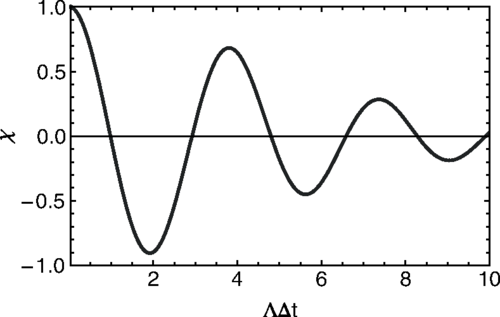
\includegraphics[width=.6\linewidth]{./graphics/FIG.2.png}
\end{center}
\item The solution is modified (at late time) to be
\begin{equation}
\rfun{a}{t,\vec x} \approx \ee^{\int_0^t \rfun{\hH_{\vec x}}{t'}\,\dd t'}
\rfun{P}{t,\vec x},
\label{eq:approx-a}
\end{equation}
where $\rfun{P}{t,\vec x}$ behaves also only quasi-periodically (see below).

\end{itemize}

\end{frame}

\begin{frame}{Proper distance and Hubble parameter revisited}
\begin{itemize}
\item The expressions for proper distance and Hubble parameter in terms of 
\cref{eq:approx-a} are
\begin{align}
\rfun{L}{1 \to 2; t} &= \rfun{L}{0}\,\ee^{\hH t},\\
\rfun{L}{1 \to 2; 0} &= \int_{\vec x_1}^{\vec x_2} \sqrt{\rfun{P^2}{t,\vec 
x}}\,\dd t,\\
\hH &= \frac{1}{t} \int_0^t \rfun{\hH_{\vec x}}{t'}\,\dd t'.
\end{align}
\item It looks like that the authors assumed averaging $\hH_{\vec x}$ over a 
long time smooths out the difference between different $\vec x$.

\item $P$ and $L$ can be solved by WKB; the presentation will focus on $\hH$
\end{itemize}

\end{frame}



\section{Solving $\rfun{a}{t,\vec{x}}$: adiabatic approximation}

\begin{frame}{Review: canonical transformation}
\begin{itemize}
\item Introducing the (type-2) generating function $\rfun{G_2}{q, P, t}$
\begin{equation}
S = \int p\,\dd q - H \,\dd t
\equiv \int P\,\dd Q - K\,\dd t + \dd \rbr{-QP + G_2}
\end{equation}
where $H = \rfun{H}{q, p, t}$, $K = \rfun{K}{Q, P, t}$, so that
\begin{equation}
\int \rbr{p - \partial_q G_2}\,\dd q + \rbr{Q - \partial_P G_2}\,\dd P 
+ \rbr{K - H + \partial_t G_2}\,\dd t\equiv 0.
\end{equation}
\item Arbitrariness of the track in phase space requires
\begin{equation}
p = \partial_q G_2,\quad
Q = \partial_P G_2,\quad
K = H - \partial_t G_2.
\end{equation}
\item It can be shown that $G_2$ generates a Possion-bracket-keeping 
transformation from $\rbr{q, p; H}$ to $\rbr{Q, P; K}$.
\end{itemize}
\end{frame}

\begin{frame}{Action-angle variables}
\begin{itemize}
\item Consider a $\rfun{G_2}{q, J}$ which brings $\rbr{q, p; \rfun{H}{q, p}}$ 
to $\rbr{\varphi, I; \rfun{K}{I}}$; note the time-independence
\item Dynamics in the new variables reads
\begin{alignat}{3}
\dot \varphi &= \partial_I K,&\quad \dot I &= 0; \\
\Rightarrow \varphi &= \rbr{\partial_I K}\,t+\varphi_0,&\quad I &\equiv I_0
\end{alignat}
\item $G_2$ can be solved by the Hamilton--Jacobi-like equation
\begin{equation}
\rfun{H}{q, \partial_q G_2} = \rfun{K}{J}.
\end{equation}
\item If the motion has a period $T$ and it requires $\Delta \varphi \coloneqq 
\rbr{\partial_I K}\,T \equiv 2\pp$ (angle variable), it can be shown that
\begin{equation}
I = \frac{1}{2\pp}\oint p\,\dd q,
\end{equation}
thus the name action-angle variable comes.


\end{itemize}
\end{frame}

\begin{frame}{Adiabatic approximation}
\begin{itemize}
\item The variables above can be extended to $H = \rfun{H}{q, p; \lambda}$; 
where a perturbative expansion is made in terms of $\epsilon = \dd \lambda / \dd 
t$.
\item It can be shown that the leading-order expansion gives
\begin{equation}
\vbr{\rfun{I}{t} - \rfun{I}{0}} \le C \epsilon,\quad 0 \le t \le \epsilon^{-1}
\end{equation}
\item Let $\omega$ be the angular frequency of the unperturbed system. If
\begin{equation}
\lambda^{-1} \epsilon \ll \omega,
\end{equation}
then $I$ varies only slightly during one quasi-period $2\pp/\omega$ and is 
thus a good \alert{adiabatic invariance}.

\end{itemize}

\end{frame}



\section*{Summary}

\begin{frame}{Summary}

  % Keep the summary *very short*.
\begin{itemize}
\item
Compared the \alert{pure} and the \alert{thermal} descriptions of the
radiation within the solvable dilaton gravity model
\item
Fourier-mode fluctuation: that of the thermal state \alert{diverges} faster
than the vacuum case does at low energy, while the pure-state fluc.\ remains
\alert{finite}; at high energies they \alert{converge}.
\item
Trace distance: goes exponentially \alert{small} with black hole 
\alert{temperature} going to zero.
\end{itemize}
  
  % The following outlook is optional.
  \vskip0pt plus.5fill
  \begin{itemize}
  \item
	Outlook in the proposed PhD study
	\begin{itemize}
	\item Further discussion within full CGHS, BTZ, etc.
	\item Make use of the decoherence theory
	\end{itemize}
	\begin{itemize}
	\item Nature of the microscopic degrees of freedom for BH entropy
	\item Breakdown of the semi-classical approximations in QG
    \end{itemize}
%	\item Understand the dilaton gravity model
%	\item Understand the Fourier-mode fluctuation
%	\item Evaluate the real space correlator
%	\item Understand practical meaning of trace distance
%	\item Understand the regulator in total trace distance
%	\item Evaluate the exact trace distance
%	\item Include the gravitational wave functional
  \end{itemize}
\end{frame}



% All of the following is optional and typically not needed. 
\appendix
\section<presentation>*{\appendixname}
\subsection<presentation>*{For Further Reading}

\begin{frame}[allowframebreaks]
  \frametitle<presentation>{For Further Reading}
    
%  \begin{thebibliography}{10}
    
  \beamertemplatebookbibitems
  % Start with overview books.
\printbibliography[type=book]

%  \bibitem{Author1990}
%    A.~Author.
%    \newblock {\em Handbook of Everything}.
%    \newblock Some Press, 1990.
 
    
  \beamertemplatearticlebibitems
  % Followed by interesting articles. Keep the list short. 
\printbibliography[nottype=book]

%  \bibitem{Someone2000}
%    S.~Someone.
%    \newblock On this and that.
%    \newblock {\em Journal of This and That}, 2(1):50--100,
%    2000.
%  \end{thebibliography}
\end{frame}

\section<presentation>*{More on Trace Distance and Fidelity}






\end{document}


